\documentclass[a4paper]{article}
\usepackage[utf8]{inputenc}
\usepackage[spanish, es-tabla]{babel}

\usepackage[a4paper, footnotesep = 1cm, width=18cm, left=2cm, top=2.5cm, height=25cm, textwidth=18cm, textheight=25cm]{geometry}
%\geometry{showframe}

\usepackage{tikz}
\usepackage{amsmath}
\usepackage{amsfonts}
\usepackage{amssymb}
\usepackage{float}
\usepackage{graphicx}
\usepackage{caption}
\usepackage{subcaption}
\usepackage{multicol}
\usepackage{multirow}
\setlength{\doublerulesep}{\arrayrulewidth}
\usepackage{xcolor}

\usepackage{hyperref}
\hypersetup{
    colorlinks=true,
    linkcolor=blue,
    filecolor=magenta,      
    urlcolor=blue,
    citecolor=blue,    
}

\newcommand{\quotes}[1]{``#1''}
\usepackage{array}
\newcolumntype{C}[1]{>{\centering\let\newline\\\arraybackslash\hspace{0pt}}m{#1}}
\usepackage[american]{circuitikz}
\usepackage{fancyhdr}
\usepackage{units} 

\pagestyle{fancy}
\fancyhf{}
\lhead{22.13 Electrónica III}
\rhead{Mechoulam, Lambertucci, Martorell, Londero}
\rfoot{\center \thepage}
 
\begin{document}
\subsection{Introducción}

En el presente ejercicio se procedio a medir los tiempos de propagación, rise y fall de una compuerta NOR del IC 74HC02 primero al vacio y luego implementando el siguiente circuito y distintas modificaciones a este último:

\begin{figure}[h]
    \centering
    
\includegraphics{ImagenesEjercicio4/pend.jpg}
    \caption{Circuito a implementar}
\end{figure}

\subsection{Mediciones a baja frecuencia}

Primero se realizaron las mediciones utilizando un escalón de amplitud $V_{pp}=5V$ con una frecuencia $f=5 Hz$ y se obtuvo los siguientes resultados:

\begin{table}[H]
\centering
\begin{tabular}{|c|c|c|c|c|}
\hline
Caso & $tpd_{L-H}(ns)$ & $tpd_{H-L}(ns)$ & trise$(ns)$ & tfall$(ns)$ \\ \hline
Sin carga & 11.10 & 8.75 & 21.0 & 19.0 \\ \hline
Con carga & 12.30 & 9.45 & 22 & 19.8 \\ \hline
%Sin carga (100 kHz) & 8.35 & 9.85 & 19.6 & 19.1 \\ \hline
%Con carga (100 kHz) & 12.15 & 9.25 & 20 & 19.4 \\ \hline
%Con carga y capacitores (100 kHz) & 15.85 & 12.60 & 25 & 25.1 \\ \hline
\end{tabular}
\end{table}

Tomando en cuenta las limitaciones presentadas por el osciloscopio disponible en el laboratorio se puede apreciar que los tiempos medidos se asemejan bastante a los de sus análogos establecidos en la hoja de datos provista por el fabricante. En frecuencias bajas al conectar la carga  ya establecida se puede apreciar que sus tiempos de operación se incrementan levemente alrededor de $1 ns$. 

\subsection{Mediciones a alta frecuencia}
Acontinuación se procedio a aumentar la frecuencia de la señal de entrada a $f=100 kHz$ y se repetieron las mediciones previamente obteniendo los siguientes resultados:


\begin{table}[H]
\centering
\begin{tabular}{|c|c|c|c|c|}
\hline

Caso & $tpd_{L-H}(ns)$ & $tpd_{H-L}(ns)$ & trise$(ns)$ & tfall$(ns)$ \\ \hline
Sin carga (100 kHz) & 8.35 & 9.85 & 19.6 & 19.1 \\ \hline
Con carga (100 kHz) & 12.15 & 9.25 & 20 & 19.4 \\ \hline
\end{tabular}
\end{table}

En donde otra vez se puede observar que la compuerta tarda mas en actuar si se encuentra conectada a una carga, además a mayor frecuencia se puede notar que el integrado tuvo un leve aumento en su temperatura, esto se debe a que al tener transicionar con mayor velocidad entre estado alto y bajo los transistores permanecen mas tiempo en la zona activa por lo que consumen mayor potencia que se manifiesta como el aumento de temperatura previamente mencionado.

\subsection{Mediciones a la tensión de alimentación}
Con el circuito trabajando con una señal de entrada de frecuencia $f=100 kHz$ se ve se puede notar que al realizarse una transción de estados la alimentación experimenta un sobrepico seguido de un régimen subamortiguado hasta que vuelve a establecerse despues de cierto tiempo. Se puede notar que antes de dicho sobrepico la tensión decae por debajo de los $4V$ y aumenta hasta llegar al rededor de los $5.5V$ esto fenómeno ocurre debido a la compuerta que le pide mas corriente a la alimentación en dichas transiciones.
Para solucionar este problema el fabricante recomienda poner capacitores de desacople de $100 nf$ entre las terminales de alimentación del integrado y la alimentación del circuito tratando de que esten lo mas cercanos posibles dichas terminales. Una vez colacado dichos capacitores se puede observar en la siguiente figura una considerable reducción tanto al sobrepico como al tiempo de establecimiento que se observaban anteriormente.



\begin{figure}[H]
    \centering
    \begin{tabular}{c c}
        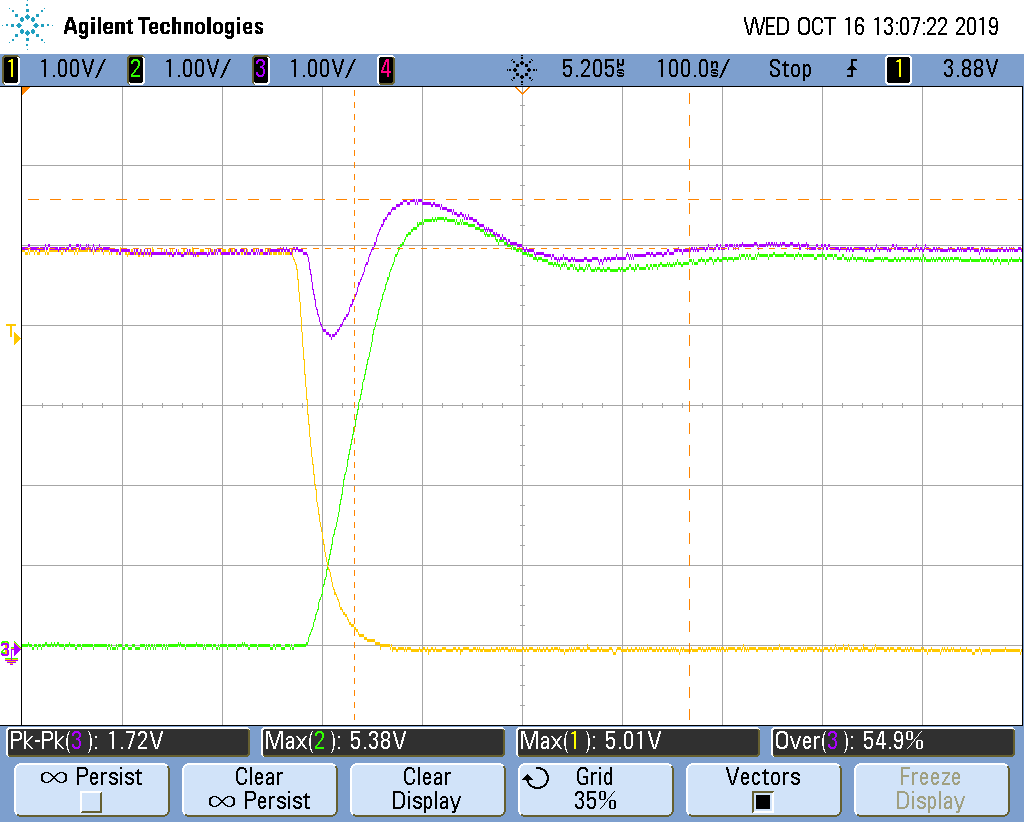
\includegraphics[width=0.4\textwidth]{ImagenesEjercicio4/overshoot.png} &
        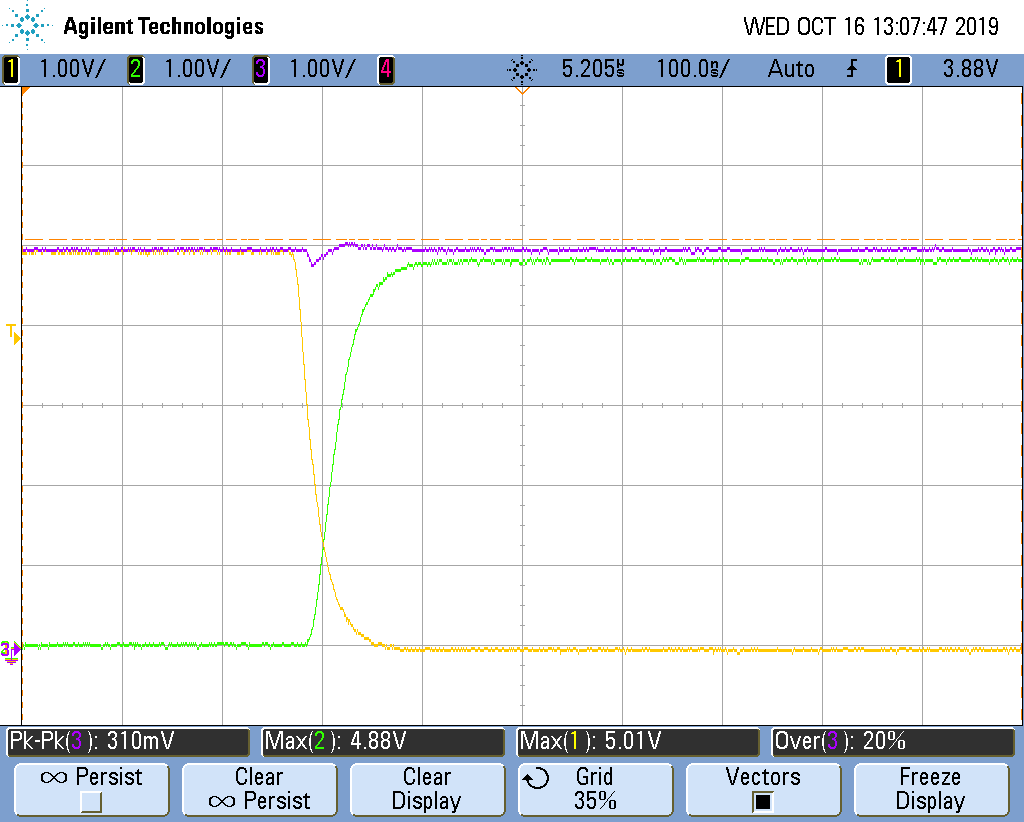
\includegraphics[width=0.4\textwidth]{ImagenesEjercicio4/overshoot_c.png}
    \end{tabular}
    \caption{Medición de alimentación primero sin y despues con compensación, en amarillo la señal de entrada, en verde la señal de salida y en azul la alimentación}
    
\end{figure}



\end{document}